\documentclass[letterpaper]{article}\usepackage[]{graphicx}\usepackage[]{color}
%% maxwidth is the original width if it is less than linewidth
%% otherwise use linewidth (to make sure the graphics do not exceed the margin)
\makeatletter
\def\maxwidth{ %
  \ifdim\Gin@nat@width>\linewidth
    \linewidth
  \else
    \Gin@nat@width
  \fi
}
\makeatother

\definecolor{fgcolor}{rgb}{0, 0, 0}
\newcommand{\hlnum}[1]{\textcolor[rgb]{0.502,0,0.502}{\textbf{#1}}}%
\newcommand{\hlstr}[1]{\textcolor[rgb]{0.651,0.522,0}{#1}}%
\newcommand{\hlcom}[1]{\textcolor[rgb]{1,0.502,0}{#1}}%
\newcommand{\hlopt}[1]{\textcolor[rgb]{1,0,0.502}{\textbf{#1}}}%
\newcommand{\hlstd}[1]{\textcolor[rgb]{0,0,0}{#1}}%
\newcommand{\hlkwa}[1]{\textcolor[rgb]{0.733,0.475,0.467}{\textbf{#1}}}%
\newcommand{\hlkwb}[1]{\textcolor[rgb]{0.502,0.502,0.753}{\textbf{#1}}}%
\newcommand{\hlkwc}[1]{\textcolor[rgb]{0,0.502,0.753}{#1}}%
\newcommand{\hlkwd}[1]{\textcolor[rgb]{0,0.267,0.4}{#1}}%

\usepackage{framed}
\makeatletter
\newenvironment{kframe}{%
 \def\at@end@of@kframe{}%
 \ifinner\ifhmode%
  \def\at@end@of@kframe{\end{minipage}}%
  \begin{minipage}{\columnwidth}%
 \fi\fi%
 \def\FrameCommand##1{\hskip\@totalleftmargin \hskip-\fboxsep
 \colorbox{shadecolor}{##1}\hskip-\fboxsep
     % There is no \\@totalrightmargin, so:
     \hskip-\linewidth \hskip-\@totalleftmargin \hskip\columnwidth}%
 \MakeFramed {\advance\hsize-\width
   \@totalleftmargin\z@ \linewidth\hsize
   \@setminipage}}%
 {\par\unskip\endMakeFramed%
 \at@end@of@kframe}
\makeatother

\definecolor{shadecolor}{rgb}{.97, .97, .97}
\definecolor{messagecolor}{rgb}{0, 0, 0}
\definecolor{warningcolor}{rgb}{1, 0, 1}
\definecolor{errorcolor}{rgb}{1, 0, 0}
\newenvironment{knitrout}{}{} % an empty environment to be redefined in TeX

\usepackage{alltt}
%\VignetteIndexEntry{Multilocus Genotype Analysis}
%\VignetteEngine{knitr::knitr}
\usepackage{graphicx}
\usepackage[colorlinks = true,
            urlcolor = blue,
            citecolor = blue,
            linkcolor = blue]{hyperref}
\usepackage{array}
\usepackage{color}
\usepackage[usenames,dvipsnames,svgnames,table]{xcolor}
\usepackage[utf8]{inputenc} % for UTF-8/single quotes from sQuote()
\usepackage{fullpage}
\usepackage{mathtools}
\usepackage{makeidx}
\usepackage{longtable}
\usepackage{natbib}

% for bold symbols in mathmode
\usepackage{bm}
\newcommand{\R}{\mathbb{R}}
\newcommand{\m}[1]{\mathbf{#1}}
\newcommand{\tab}{\hspace*{1em}}
\newcolumntype{H}{>{\setbox0=\hbox\bgroup}c<{\egroup}@{}}
\newcommand{\cmdlink}[2]{%
  \texttt{\hyperref[#1]{#2}}%
}
\newcommand{\seclink}[2]{%
  \textsc{\hyperref[#1]{#2}}%
}

\newcommand{\poppr}{\textit{poppr}}
\newcommand{\Poppr}{\textit{Poppr}}
\newcommand{\adegenet}{\textit{adegenet}}
\newcommand{\Adegenet}{\textit{Adegenet}}
\newcommand{\tline}{
  \noindent
  \rule{\textwidth}{1pt}
  \par
}
\newcommand{\bline}{
  \noindent
  \rule{\textwidth}{1pt}
  \kern1pt
}

\newcommand{\jala}{
  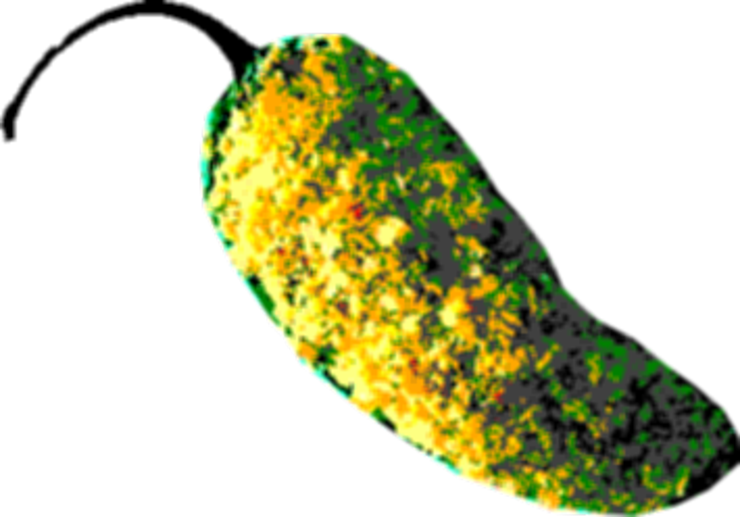
\includegraphics[height = 5mm, keepaspectratio=true]{jalapeno-poppers}
}

\newcommand{\revjala}{
  \scalebox{-1}[1]{\jala{}}
}

\title{Analysis of Multilocus Genotypes and Lineages in 1.1.5.99.583}

\author{Zhian N. Kamvar$^{1}$\ and Niklaus J. Gr\"unwald$^{1,2}$\\\scriptsize{1)
Department of Botany and Plant Pathology, Oregon State University, Corvallis,
OR}\\\scriptsize{2) Horticultural Crops Research Laboratory, USDA-ARS,
Corvallis, OR}}
\IfFileExists{upquote.sty}{\usepackage{upquote}}{}
\begin{document}


\maketitle

\begin{abstract}
A multilocus genotype is the unique combination of alleles across two or more
loci. For organisms such as plant pathogens that often reproduce clonally,
mulitlocus genotypes are invaluable for identifying the mode and spread of an
organism. This document will describe in detail how you can define multilocus
genotypes/lineages and how you can use them for your analyses.

\end{abstract}

\begin{figure}[b]   
  \centering
  \label{logo}   
  
\includegraphics{popprlogo} 
\end{figure} 

\newpage 
\begingroup
  \hypersetup{linkcolor=black} 
  \tableofcontents 
\endgroup 


\section{Introduction}
\label{intro}
%==============================================================================%
%==============================================================================%


\section{Multilocus Genotype Flavors}
\label{type}
%==============================================================================%
%==============================================================================%
There are three different way for constructing multilocus genotypes in \poppr{}.
The first is a simply na\"ive construction where all alleles must match to make
a unique multilocus genotype. New in version 1.1.5.99.583 is
the ability to use genetic distance to define multilocus genotypes or define
custom multilocus genotypes based on other biological factors. In this section,
we will demonstrate how to construct each of these three multilocus genotype
definitions in different data sets.

\subsection{Na\"ive}
\label{type:naive}

The na\"ive definition simply takes strings of alleles and compares them for
equality. This method is quick and easily interpretable, but means that things
like genotyping error, hyper-variable loci, and missing data all contribute to a
unique genotype that might not be truly unique \citep{kamvar2015novel}.


\subsection{Filtered}
\label{type:filter}

\subsection{Custom}
\label{type:custom}


\section{Diversity Analysis}
\label{diversity}
%==============================================================================%
%==============================================================================%

\section{Clone Correction}
\label{cc}
%==============================================================================%
%==============================================================================%

\section{Conclusions}
\label{conclusion}
%==============================================================================%
%==============================================================================%

\bibliographystyle{authordate1}
\bibliography{the_bibliography}
\end{document}
